\documentclass{article}
\usepackage[margin=1in]{geometry}
\usepackage{hyperref}
\usepackage{amsmath,amsfonts,amssymb,amsthm,commath,dsfont}
\usepackage{enumitem}
\usepackage{bbold}
\usepackage{amsmath}
\usepackage{framed}
\usepackage{xspace}
\usepackage{booktabs}
\usepackage{microtype}
\usepackage{float}
\usepackage[round]{natbib}
\usepackage{cleveref}
\usepackage[dvipsnames]{xcolor}
\usepackage{graphicx}
\usepackage{listings}
\usepackage[breakable]{tcolorbox}
\tcbset{breakable}
\usepackage{bbm}
\usepackage{mathtools, bm}
%\usepackage{symbols}
\usepackage{subcaption}
\usepackage{url}
        
\usepackage{pifont}
\newcommand{\cmark}{\ding{51}}
\newcommand{\xmark}{\ding{55}}
\newcommand{\vect}[1]{\boldsymbol{#1}}
\newcommand{\colbar}{\rule[-3mm]{.3mm}{1.5em}}
\newcommand{\rowbar}{\rule[.5ex]{1.5em}{.3mm}}
\DeclareMathOperator{\rank}{rank}
\DeclareMathOperator*{\argmax}{argmax}
\DeclareMathOperator*{\argmin}{argmin}

% following loops stolen from djhsu
\def\ddefloop#1{\ifx\ddefloop#1\else\ddef{#1}\expandafter\ddefloop\fi}
% \bbA, \bbB, ...
\def\ddef#1{\expandafter\def\csname bb#1\endcsname{\ensuremath{\mathbb{#1}}}}
\ddefloop ABCDEFGHIJKLMNOPQRSTUVWXYZ\ddefloop
        
% \cA, \cB, ...
\def\ddef#1{\expandafter\def\csname c#1\endcsname{\ensuremath{\mathcal{#1}}}}
\ddefloop ABCDEFGHIJKLMNOPQRSTUVWXYZ\ddefloop
        
% \vA, \vB, ..., \va, \vb, ...
\def\ddef#1{\expandafter\def\csname v#1\endcsname{\ensuremath{\boldsymbol{#1}}}}
\ddefloop ABCDEFGHIJKLMNOPQRSTUVWXYZabcdefghijklmnopqrstuvwxyz\ddefloop
        
% \valpha, \vbeta, ...,  \vGamma, \vDelta, ...,
\def\ddef#1{\expandafter\def\csname v#1\endcsname{\ensuremath{\boldsymbol{\csname #1\endcsname}}}}
\ddefloop {alpha}{beta}{gamma}{delta}{epsilon}{varepsilon}{zeta}{eta}{theta}{vartheta}{iota}{kappa}{lambda}{mu}{nu}{xi}{pi}{varpi}{rho}{varrho}{sigma}{varsigma}{tau}{upsilon}{phi}{varphi}{chi}{psi}{omega}{Gamma}{Delta}{Theta}{Lambda}{Xi}{Pi}{Sigma}{varSigma}{Upsilon}{Phi}{Psi}{Omega}{ell}\ddefloop

\newcommand{\liangyan}[1]{\textcolor{blue}{[{\bf Liangyan:} #1]}}


\newcommand\T{{\scriptscriptstyle\mathsf{T}}}
\def\diag{\textup{diag}}
        
\def\SPAN{\textup{span}}
\def\tu{\textup{u}}
\def\R{\mathbb{R}}
\def\E{\mathbb{E}}
\def\Z{\mathbb{Z}}
\def\be{\mathbf{e}}
\def\nf{\nabla f}
\def\veps{\varepsilon}
\def\cl{\textup{cl}}
\def\inte{\textup{int}}
\def\dom{\textup{dom}}
\def\Rad{\textup{Rad}}
\def\lsq{\ell_{\textup{sq}}}
\def\hcR{\widehat{\cR}}
\def\hcRl{\hcR_\ell}
\def\cRl{\cR_\ell}
\def\hcE{\widehat{\cE}}
\def\cEl{\cE_\ell}
\def\hcEl{\hcE_\ell}
\def\eps{\epsilon}
\def\1{\mathds{1}}
\newcommand{\red}[1]{{\color{red} #1}}
\newcommand{\blue}[1]{{\color{blue} #1}}
\def\srelu{\sigma_{\textup{r}}}
\def\vsrelu{\vec{\sigma_{\textup{r}}}}
\def\vol{\textup{vol}}

\newcommand{\ip}[2]{\left\langle #1, #2 \right \rangle}
\newcommand{\mjt}[1]{{\color{blue}\emph\textbf{[M:}~#1~\textbf{]}}}
\newcommand{\sahand}[1]{{\color{green}\emph\textbf{[Sah:}~#1~\textbf{]}}}
		
\newtheorem{fact}{Fact}
\newtheorem{lemma}{Lemma}
\newtheorem{condition}{Condition}
\theoremstyle{definition}
\theoremstyle{remark}
\newtheorem{remark}{Remark}
\newtheorem{example}{Example}

\newenvironment{Q}
{%
    \clearpage
    \item
}
{%
    \phantom{s} %lol doesn't work
    \bigskip
    \textbf{Solution.}
}

\title{CS 446 / ECE 449 --- Homework 5}
\author{\emph{your NetID here}}
\date{Version 1.0}

\begin{document}
\maketitle

\noindent\textbf{Instructions.}
\begin{itemize}
   \item
            Homework is due \textbf{Wednesday, Nov. 17th, at noon CST}; you have \textbf{3} late days in total for \textbf{all Homeworks}.
        
          \item
            Everyone must submit individually at gradescope under \texttt{hw5} and \texttt{hw5code}.
        
          \item
            The ``written'' submission at \texttt{hw5} \textbf{must be typed}, and submitted in
            any format gradescope accepts (to be safe, submit a PDF).  You may use \LaTeX, markdown,
            google docs, MS word, whatever you like; but it must be typed!
        
          \item
            When submitting at \texttt{hw5}, gradescope will ask you to \textbf{mark out boxes
            around each of your answers}; please do this precisely!
        
          \item
            Please make sure your NetID is clear and large on the first page of the homework.
        
          \item
            Your solution \textbf{must} be written in your own words.
            Please see the course webpage for full \textbf{academic integrity} information.
            You should cite any external reference you use.
        
          \item
            We reserve the right to reduce the auto-graded score for
            \texttt{hw5code} if we detect funny business (e.g., your solution
            lacks any algorithm and hard-codes answers you obtained from
            someone else, or simply via trial-and-error with the autograder).
            
          \item
           When submitting to \texttt{hw5code}, only upload \texttt{hw5.py}. Additional files will be ignored.
        
\end{itemize}
        
       
\begin{enumerate}[font={\Large\bfseries},left=0pt]


\begin{Q}
\textbf{\Large Expectation Maximization}

In this question, we expect you to do some computation related to the EM algorithm covered in the lecture.

\textbf{Background.} On the xy-plane, we have a rigid object, and our sensor can capture $N$ key points, whose coordinates are: $\mathcal{P}=\{\vp^{(1)}, \vp^{(2)}, ..., \vp^{(N)}\}$. ($N$ is a sufficiently large integer.) An unknown force then cause a translation $\mathbf{T}$ to this object, where $\mathbf{T}$ is encoded $T_x$ and $T_y$, meaning how long the object has moved along the x-axis and y-axis. To calculate parameter $\mathbf{T}$, we use our sensor to capture the key points on the rigid object one more time, acquiring a set of $N$ key points: $\mathcal{Q}=\{\vq^{(1)}, \vq^{(2)}, ..., \vq^{(N)}\}$. (See Fig.~\ref{fig:em} for an intuitive demonstration. The ``L'' is our rigid body, $N=3$, and the blue and red dots are the key points.)

\textbf{Assumption.} During this process, we assume that an bi-jection mapping between $\mathcal{P}$ and $\mathcal{Q}$ exists (See Fig.~\ref{fig:em}, the key points are all the corners of ``L.'') However, this bijection mapping cannot be directly got from the sensors, as the orders of the points may be shuffled during perception. 

\begin{figure}[h]
    \centering
    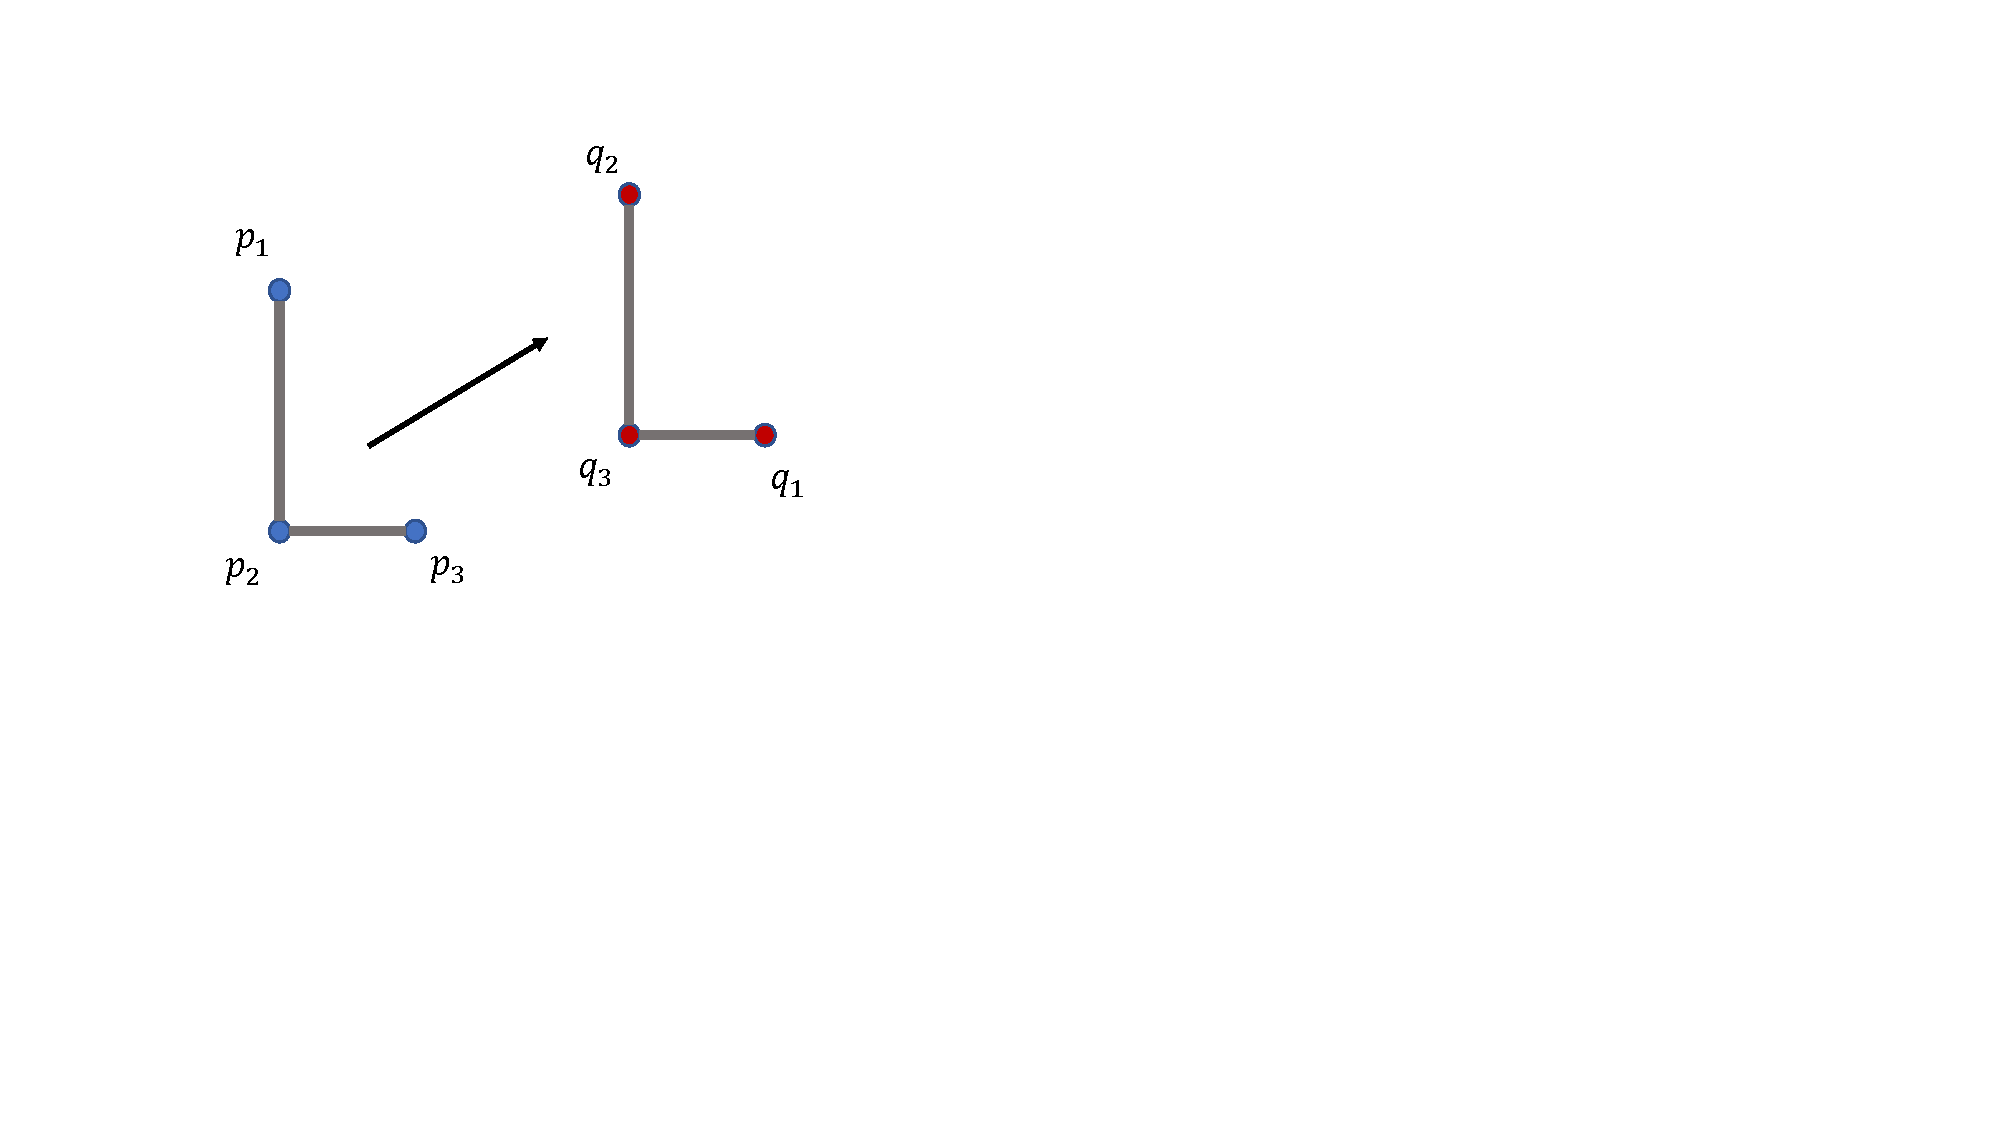
\includegraphics[width=0.6\columnwidth]{figs/em.pdf}
    \caption{}
    \label{fig:em}
\end{figure}

\textbf{Objective.} Using EM algorithm to estimate the translation parameter and the corresponding pairs of ke points, by introducing binary hidden variables $\vZ \in \mathbb{R}^{N\times N}$, where $Z_{ij}=1$ means  $\vp^{(i)}$ and $\vq^{(j)}$ are a match.

\textbf{Remark.} We have the following remarks on this question.

\begin{itemize}[itemsep=-1mm]
    \item This questions set is for you to understand the process of EM with an intuitive example without annoying mathematical equations. However, to make it easy to understand, we use additional assumptions and simplifications. Please note the difference between this example and rigorous EM algorithm when you learn deeper machine learning courses in the future.
    \item You may find EM overkill for this simple question, and you are right about it. This question originates from a classical problem in computer vision called ``point cloud registration,'' where this problem could be much more difficult when the sensor has noises and the bijection between $\mathcal{P}$ and $\mathcal{Q}$ does not exist. You may refer to ``iterative closest points'' (ICP) if you are interested in this.
\end{itemize}

\begin{enumerate}

\item \textbf{Joint Probability.} 
If we know a pair of \textbf{matched} points $(\vp^{(i)}, \vq^{(j)})$, think of it as a single data sample, with the corresponding hidden state $Z_{ij}=1$. Intuitively, based on this single pair, how likely parameter $\vT$ is depends on $\|\vp^{(i)}+\vT-\vq^{(j)}\|_2$. To make the math easier, we assume $\|\vp+\vT-\vq\|_2$ follows from the Gaussian distribution $\mathcal{N}(0, \sigma)$ where $\sigma$ is known, i.e.,

\begin{equation}
    \mathbb{P}_{\vT}((\vp^{(i)}, \vq^{(j)})|Z_{ij}=1)=\frac{1}{\sqrt{2\pi} \sigma}\exp(-{\frac{\|\vp^{(i)}+\vT-\vq^{(j)}\|_2^2}{2\sigma^2}})
    \label{eq:em_gaussian}
\end{equation}
(To avoid confusion in the notations,  please use $\mathbb{P}$ to represent probability)

But we actually don't know which points are a match, or say we don't know the hidden states $\vZ$, and want to use EM to help. We define that the matching is optimized from $\mathcal{P}$ to $\mathcal{Q}$, and not the reverse. In this way, the matching between each point $\vp\in\mathcal{P}$ is independent, and two points $\vp\in\mathcal{P}$ can match to the same $\vq\in\mathcal{Q}$, but not the reverse.

Let $\mathbb{P}(Z_{ij}=1):=\Pi_{ij}$ indicate the prior probability of $\vp^{(i)}$ and $\vq^{(j)}$ being a pair, where $\vPi\in\mathbb{R}^{N\times N}$ are unknown parameters. Under our assumption, $0 \leq \Pi_{ij} \leq 1$, and $\sum_{k=1}^{N} \Pi_{ik}=1, \forall\ i\in\{1,2,...,N\}$. Let us denote overall parameters $(\vT, \vPi)$ as $\psi$ like in the class.

Given a point $\vp^{(i)}$, it has $N$ possible matches $\vq^{(j)}, j=1,...,N$. The probability contributed by $\vp^{(i)}$ in the complete data likelihood is

\begin{equation}
    \mathbb{P}(\vp^{(i)},\mathcal{Q},\vZ_{i,:})=\mathbb{P}(\vp^{(i)},\mathcal{Q}|\vZ_{i,:})\mathbb{P}(\vZ_{i,:})= \prod_{j=1}^{N}[\mathbb{P}_\psi((\vp^{(i)}, \vq^{(j)})|Z_{ij}=1)\mathbb{P}(Z_{ij}=1)]^{Z_{ij}}
\end{equation}

\textbf{Please write the log-likelihood $\log{\mathbb{P}_{\psi}(\mathcal{P}, \mathcal{Q}, \vZ)}$ under the two following cases.}

\begin{enumerate}
    \item General Case: Write out the general formula for $\log{\mathbb{P}_{\psi}(\mathcal{P}, \mathcal{Q}, \vZ)}$ following the ``Log-likelihood of complete data'' on Slides 7/27 in lecture 17.
    \item Special Case: $Z_{ii}=1, i\in\{1,2,3.., N\}$. To get the full credits of this question, please full expand the Gaussian distributions.
\end{enumerate}

\item \textbf{Expectation. (1/2)} After doing the preparation work, we now start to apply EM algorithm to this question. In the E-step, our first objective is to compute $\vR$, where $\vR=[r_{ij}]\in\mathbb{R}^{N\times N}$, and $r_{ij}=\mathbb{P}_{\psi^{(t)}}(Z_{ij}|\vp^{(i)}, \mathcal{Q})$.

Following the procedure of ``the first line of the E-step on slides 8/27 in lecture 17,'' answer the following questions.

\begin{enumerate}
    \item General Case: Derive the formula for $r_{ij}$. For the simplicity of notations, you can also use $\mathcal{N}(\cdot|\cdot, \cdot)$ like on the slides to denote Gaussian distribution.
    \item Special Case: For the $N$ points in $\mathcal{P}$, the first $[\frac{N}{2}]$ points are matched with $\vq^{(1)}$, and the rest are matched to $\vq^{(2)}$. Write the values of $\bm{R}$.
\end{enumerate}

\item \textbf{Expectation. (2/2)} This question computes the values of $Q(\psi|\psi^{(t)})$. Please answer the following questions.

\begin{enumerate}
    \item General Case: Derive the formula of $Q(\psi|\psi^{(t)})$ following the procedure on slides 8/27 in lecture 17. For the simplicity of notations, you can also use $\mathcal{N}(\cdot|\cdot, \cdot)$ to denote Gaussian distribution.
    
    \item Special Case: Same as the special case mentioned in problem ``Expectation (1/2),'' fully expand the formula of $Q(\psi|\psi^{(t)}$. To get full credits, your answer cannot have the variables $r_{ij}$ and the notation for Gaussian distribution $\mathcal{N}(\cdot|\cdot, \cdot)$. (use $0 \times \log 0 =0 $ in your calculation)

\end{enumerate}

\item \textbf{Maximization.} On the basis of previous derivation, complete the maximization step and the update rule. Similar to the slides 9/27 in lecture 17, write out the formulas for $\vPi^{(t+1)}$ and $\vT^{(t+1)}$.

\textbf{Hint.} $\sigma$ is fixed and you do not need to solve it.

\begin{enumerate}
\item General Case: Write the formulas for $\vPi^{(t+1)}$ and $\vT^{(t+1)}$. You may use $N$, $\vR$, and the points in $\mathcal{P}$ and $\mathcal{Q}$.

\item Special Case: Write the formulas for $\vT^{(t+1)}$ for the special case in question ``Expectation (1/2).'' You may use $N$, and the points in $\mathcal{P}$ and $\mathcal{Q}$.

\end{enumerate}

\end{enumerate}
\end{Q}
          
\begin{Q}
\textbf{\Large Variational Auto-Encoders}\\

We are training a variational auto-encoder (VAE). It contains the following parts: the input are vectors $\vx$, the latent vector is $\vz$, the encoder models the probability of $q_{\phi}(\vz|\vx)$, and the decoder is $p_{\theta}(\vx|\vz)$. Based on this notation, we will first look at several problems related to the structure of variational auto-encoder.

\begin{enumerate}

\item We assume the latent vector $\vz \in \mathbb{R}^{2}$ follows a multi-variate Gaussian distribution $\mathcal{N}$. Please compute the output dimension of the encoder $q_{\phi}(\cdot)$ under the following cases and briefly explain why. (If ``output dimension'' is not clear enough for you, think of it as ``how many real numbers $r\in \mathbb{R}$ are needed to output for the sampling of latent vectors.'')

\begin{itemize}
    \item We assume $\mathcal{N}$ follows a multi-variate Gaussian distribution with an \textbf{identity matrix} as the covariance matrix.
    \item We assume $\mathcal{N}$ follows a multi-variate Gaussian distribution with an \textbf{diagonal matrix} as the covariance matrix.
\end{itemize}

\item
We then consider the problems related to the understanding of KL-Divergence.

\begin{enumerate}
    \item Using the inequality of $\log(x) \leq x - 1$, prove that $D_{KL}(p(x), q(x))\ge 0$ holds for two arbitrary distributions $p(x)$ and $q(x)$.
    
    \item Consider a binary classification problem with input vectors $\vx$ and labels $y\in\{0, 1\}$. The distribution of the ground truth label is denoted as $P(y)$. The expression of $P(y)$ is as Eq~\ref{eq:gt}, where $y_{gt}$ is the ground truth label.
    \begin{equation}
        P(y=y_{gt})=1, P(y=1-y_{gt})=0
        \label{eq:gt}
    \end{equation}
    Suppose we are trying to predict the label of $\vx$ with a linear model $\vw$ and sigmoid function, then the distribution of $y$ is denoted as $Q(y)$ and computed as Eq.~\ref{eq:sigmoid}.
    \begin{equation}
        Q(y=0|\vx)=\frac{1}{1+\exp{(-\vw^\top \vx)}},\quad Q(y=1|\vx)=\frac{\exp{(-\vw^\top \vx)}}{1+\exp{(-\vw^\top \vx)}}
        \label{eq:sigmoid}
    \end{equation}
    
    With the above information, compute the KL Divergence between the distributions of $P(y)$ and $Q(y|\vx)$, specifically $D_{KL}(P(y), Q(y|\vx))=\mathbf{E}_{y\sim P(y)}[\log\frac{P(y)}{Q(y|\vx)}$]. 
    
    Expand your solution to the clearest form. To get full credits, your may only use $y_{gt}, \vw, \vx$ and related constants in your expression.
\end{enumerate}

\item VAE is a special branch of generative method in sampling the latent vectors $\widetilde{\vz}$ from $q_{\phi}(\vz|\vx)$ instead of directly regressing the values of $\vz$. Read an example implementation of VAE at \url{https://github.com/AntixK/PyTorch-VAE/blob/master/models/vanilla_vae.py} and answer the following questions:

\begin{enumerate}
    \item Find the functions and lines related to the sampling of $\widetilde{\vz}$ from $q_{\phi}(\vz|\vx)$. Specifying the names of the functions and the related lines can lead to full credits. Please note that if your range is too broad (in the extreme case, covering every line in the file) we cannot give your full credit.
    
    \item
    Suppose our latent variable is $\vz\in\mathbb{R}^{2}$ sampled from a Gaussian distribution with mean $\vmu\in\mathbb{R}^2$ and a diagonal covariance matrix $\vSigma=\mathtt{Diag}\{\sigma_1^2, \sigma_2^2\}$. Then another random variable $\vv\in\mathbb{R}^2$ is sampled from a Gaussian distribution $\mathcal{N}(0, \vI)$. Show that $\vV = [\sigma_1, \sigma_2]^\top \circ \vv + \vmu$ follows the same distribution as $\vz$. ($\circ$ denotes Hadamard product, which means element-wide product; $\mathcal{N}(0, \vI)$ denotes the multi-variate Gaussian with zero mean and identity matrix as covariance.)
    
    \item
    Under the same setting of the Question ii, we can sample the latent vector $\widetilde{\vz}$ by the process $\widetilde{\vz}=[\sigma_1, \sigma_2]^\top \circ \widetilde{\vv} + \vmu$, where $\widetilde{\vv}$ is a sampled random variable from $\mathcal{N}(0, \vI)$. Consider the process of training, where we apply back-propagation to train the neural networks. Given the gradient on $\widetilde{\vz}$ as $\widetilde{\vg}\in\mathbb{R}^2$, which can be written as $[\widetilde{g}_1, \widetilde{g}_2]$. \textbf{What are the gradients of the output of the encoder: $\vmu, \sigma_1, \sigma_2$?} (Assume the KL-Divergence loss is not considered in this part.)
    
    \textbf{Note:} To get full credit, you can use any constants and the variables of $\widetilde{\vv}=[\widetilde{v_1}, \widetilde{v_2}]$, $\widetilde{\vg}=[\widetilde{g}_1, \widetilde{g}_2]$, and $\vmu, \sigma_1, \sigma_2$.
    
    \item During reading the code, you might feel confused about why we are sampling $\widetilde{\vz}$ in such a way, instead of generating a random value directly. But now, you could have some clues. Please briefly explain ``Why we are sampling $\widetilde{\vz}$ with $\mathcal{N}(0, 1)$, instead of directly generating the values.''
\end{enumerate}

\end{enumerate}

\end{Q}
\begin{Q}
\textbf{\Large Generative Adversarial Networks}

Let's implement a Generative Adversarial Network(GAN) to create images of hand-written digits!

GAN consists of two parts: a generator network $G$ and a discriminator network $D$. $G$ is expected to generate a fake image from a random latent variable $\vz$, and $D$ is expected to distinguish fake images and real images. $G$ and $D$ are trained jointly with a minimax objective. In this question, we will use training data from MNIST to train our GAN, and let it produce some fake images that look like hand-written digits.

\begin{enumerate}
    \item First, let's implement the \texttt{Discriminator} network. It should take $32\times 32$ gray-scale images as input, and output the probability of each image being a real one. Its architecture is summarized in Table~\ref{table:D}.
    \begin{table}[H]
    \begin{center}
    \caption{\textbf{Discriminator Architecture}}
    \label{table:D}
    \begin{tabular}{ccccccc}
    \toprule
    Layer & Layer & Input & Output & Kernel & Stride & Padding \\
    Index & Type & Channels & Channels & Size & & \\
    \midrule
    1 & Conv2d & 1 & 16 & 3 & 1 & 1 \\
    2 & LeakyReLU \\
    3 & MaxPool & & & 2 & 2 & 0 \\
    \midrule
    4 & Conv2d & 16 & 32 & 3 & 1 & 1 \\
    5 & LeakyReLU \\
    6 & MaxPool & & & 2 & 2 & 0 \\
    \midrule
    7 & Conv2d & 32 & 64 & 3 & 1 & 1 \\
    8 & LeakyReLU \\
    9 & MaxPool & & & 2 & 2 & 0 \\
    \midrule
    10 & Conv2d & 64 & 128 & 3 & 1 & 1 \\
    11 & LeakyReLU \\
    12 & MaxPool & & & 4 & 4 & 0 \\
    \midrule
    13 & Linear & 128 & 1 \\
    14 & Sigmoid \\
    \bottomrule
    \end{tabular}
    \end{center}
    \end{table}
    A few notes:
    \begin{itemize}
        \item All Conv2d and Linear layers have bias terms. You do not have to explicitly set \texttt{Conv2d(..., bias=True)}, since it is default in PyTorch.
        \item Also, you do not need to explicitly initialize the weights in Conv2d and Linear layers. The default initialization by PyTorch is good enough.
        \item LeakyReLU is a variant of ReLU activation, which has a smaller gradient for negative inputs. Set \texttt{negative\_slope=0.2} for all LeakyReLU layers. More info about LeakyReLU at \url{https://pytorch.org/docs/stable/generated/torch.nn.LeakyReLU.html}.
        \item You need to reshape the tensor sometimes in the forward pass.
        \item Given a batch of images with shape \texttt{(batch\_size, 1, 32, 32)}, the output of this network should be a tensor with shape \texttt{(batch\_size)}, and the values in it are float numbers in $(0, 1)$. Our autograder will only be able to check the shape and range of the output, so be careful even if you have passed the test.
    \end{itemize}
    
    \item Next, we can implement the \texttt{Generator} network. It should take $128$-d vectors (sampled from a Gaussian distribution) as input, and output fake images. Its architecture is summarized in Table~\ref{table:G}. We will make use of transposed convolutional layers. Given an input, a transposed convolutional layer can produce an output with a higher resolution. Thus, we can generate a $32\times 32$ image from a vector by stacking such layers. A visualization of how transposed convolutional layers work can be found at \url{https://github.com/vdumoulin/conv\_arithmetic/blob/master/README.md}.
    \begin{table}[H]
    \begin{center}
    \caption{\textbf{Generator Architecture}}
    \label{table:G}
    \begin{tabular}{ccccccc}
    \toprule
    Layer & Layer & Input & Output & Kernel & Stride & Padding \\
    Index & Type & Channels & Channels & Size & & \\
    \midrule
    1 & ConvTranspose2d & 128 & 64 & 4 & 1 & 0 \\
    2 & LeakyReLU \\
    \midrule
    3 & ConvTranspose2d & 64 & 32 & 4 & 2 & 1 \\
    4 & LeakyReLU \\
    \midrule
    5 & ConvTranspose2d & 32 & 16 & 4 & 2 & 1 \\
    6 & LeakyReLU \\
    \midrule
    7 & ConvTranspose2d & 16 & 1 & 4 & 2 & 1 \\
    8 & Tanh \\
    \bottomrule
    \end{tabular}
    \end{center}
    \end{table}
    A few notes:
    \begin{itemize}
        \item Again, all Conv2d and Linear layers have bias terms and are initialized by the default setup.
        \item Same LeakyReLU as above, with \texttt{negative\_slope=0.2} for all LeakyReLU layers.
        \item You need to reshape the tensor sometimes in the forward pass.
        \item Given a batch of latent vectors with shape \texttt{(batch\_size, 128)}, the output of this network should be a tensor with shape \texttt{(batch\_size, 1, 32, 32)}, and the values in it are float numbers in $(-1, 1)$. Our autograder will only be able to check the shape and range of the output, so be careful even if you have passed the test.
    \end{itemize}
    
    \item In class we have learned that to jointly train the generator and discriminator, we optimize them with a minimax objective:
    \begin{align*}
        V(G, D):=\frac{1}{N}\sum_{i=1}^N\log D(\vx_i)&+\frac{1}{N}\sum_{j=1}^N\log (1-D(G(\vz_j))) \\
        \min_G\max_D\ &V(G,D)
    \end{align*}
    Here $N$ is the batch size (set to $64$ in our implementation), $\vx_i$ is a real image, $\vz_j$ is a random latent variable sampled from a Gaussian distribution, and $G(\vz_j)$ is a fake image generated from it. Note that we are taking average to approximate the expectation, since we are using SGD to optimize $G$ and $D$.
    
    Please complete the function \texttt{calculate\_V()} in \texttt{GAN}. You may (but not required to) use the binary cross entropy loss (see \url{https://pytorch.org/docs/stable/generated/torch.nn.BCELoss.html}) to simplify the implementation, but be careful about the sign and reduction method of BCELoss.
    
    \item We are ready to start training our GAN. The training pipeline is already provided in \texttt{train()}, and there is a \texttt{visualize()} function for your convenience. Train our GAN for $10$ epochs, and \textbf{include the generated images after training in your PDF submission}.

    Notes from TA:
    \begin{itemize}
        \item Training $10$ epochs takes me about an hour on my laptop without GPU support. I can see interesting images after two or three epochs.
        \item You can make use of Google Colab(\url{https://colab.research.google.com/}), where you can access GPUs freely and accelerate the training. Remember to set \texttt{Runtime->Change runtime type->Hardware accelerator}.
        \item Some random seeds may lead to degenerated results. It's OK to try a few and manually set your random seed (\texttt{torch.manual\_seed()}).
    \end{itemize}
\end{enumerate}

\end{Q}
 
\end{enumerate}


\end{document}
